\section{The purpose}
The purpose of this master thesis is to review and analyze methods for defining quotient types in Coq \cite{PragmaticQT}. In Coq, there is no built-in method for implementing such constructions. Therefore, we seek ways to define types that are similar to quotient types, where elements are considered equal if and only if they are in a quotient-defining relation. Our main focus will be on quotient types that have a normalization function, but we will also provide examples of quotient types without a computable normalization function. In Coq, setoids \cite{SetoidsInTT} are the primary way of implementing quotient-like structures. However, this thesis will concentrate on quotient types where we can use the standard equality relation defined in Coq's standard library. As a result, we will use other methods that concentrate on normalization elements and creating new types where only normalized elements exist. For this purpose, we will use subtyping, inductive types based on traces of normalization functions, and more.

\section{Prerequisites}
This thesis assumes that the reader has knowledge of basic algebraic concepts such as operations in modular groups, operations on fractions, and the Euclid algorithm. More advanced constructions, such as dividing sets by equivalence relation, are defined in this paper. The main focus of this thesis is the Coq language, so it is necessary to have a basic understanding of this language to be able to comprehend this thesis. The reader should be able to write definitions in Coq and differentiate between \mintinline{coq}{Fixpoint} and \mintinline{coq}{Definition}. Understanding how the termination checker works or knowing the universe hierarchy can aid in understanding this work fully, but it is optional. The reader is also expected to know the basic concepts of Type Theory, such as the product and sum of types. Additionally, there are optional sections including Category Theory and Homotopy Type Theory concepts. Furthermore, any advanced construction from those fields needed to comprehend these sections will be defined in this paper.

\section{Coq as a proof assistant}
Coq is a formal proof management system released under the GNU LGPL license. It was first introduced in 1984 and was based on the Calculus of Constructions, which relied on Type Theory. In 1991, Coq began using the more advanced Calculus of Inductive Constructions \cite{cic} \cite{cicOrigins}, which supports higher-order logic, dependent types, and statically typed programming, among other features, all thanks to the Curry-Howard isomorphism \cite{curry-howard}.

Coq can perform simple computations. However, it was primarily developed for program extraction. Users can use functions proven in Coq in other programming languages, such as OCaml. In the Coq type system, every term has its type, and every type has its universe. This is an essential concept, as different universes serve different purposes. There are four important universes:

\begin{description}
\item[\mintinline{coq}{Prop}] -- intends to be the universe of logical prepositions. This universe is impredicative, which means propositions can quantify over all propositions. Imprecativity allows us to write propositions that say something about all propositions. Elements of this universe are removed during code extraction. Consequently, there are limitations on eliminating proofs of prepositions during type construction.

\item[\mintinline{coq}{SProp}] -- similar to \mintinline{coq}{Prop}, this universe is also intended to contain logical prepositions. The main difference is the definitional irrelevance of propositions. Irrelevance means that proofs of the same statement in this universe are, by definition, equal.

\item[\mintinline{coq}{Set}] -- intends to be a universe for small types, like boolean values or natural numbers, but also products, subsets, and function types over these data types. Elements of this universe are expected to be preserved during code extraction. Accordingly, computations should take place in this universe.

\item[\mintinline{coq}{Type}] -- contains small and large sets like Prop and Set. Therefore, every type and universe lives in \mintinline{coq}{Type}, for example, \mintinline{coq}{Prop : Type}.
\end{description}

\begin{coq}{Hierarchy of universes}{}
 More experienced readers might notice that this definition of \mintinline{coq}{Type} is slightly wrong, leading to a contradiction. We know that no universe can contain itself \cite{TypeNotInType}. Despite this, when Coq is asked what type of \mintinline{coq}{Type} is, it will answer \mintinline{coq}{Type : Type}. In reality, there is a whole infinite hierarchy of universes in Coq, and every \mintinline{coq}{Type} has its level, which is just hidden from users for convenience. Therefore, \mintinline{coq}{Type : Type} should be read as \mintinline{coq}{Type(n) : Type(n+1)}.
\end{coq}

Coq allows users to define only functions that terminate. Sometimes it requires much work to convince Coq's termination checker that it is the case. The other consequence of this is the fact that in Coq, reasoning about partial functions is difficult. Nevertheless, later we will learn how to simulate nonterminating computations. The most significant advantage of Coq is that it has imperative tactic language, which makes proving theorems much more accessible than in languages like Agda \cite{agda} or Idris \cite{idris}.

\section{Quotient types}
Quotient type is a concept from abstract algebra \cite{AbstractAlgebra}, which has found applications in other fields like computer science.
\begin{defi}{Quotients in abstract algebra}{def:quotients_in_aa}
In abstract algebra, an underlying set $T$ partitioned by equivalence relation ($\sim$) is called a quotient and denoted $T/\sim$.
\end{defi}
\begin{example}{Clockwise operations}{ex:clock}
An excellent example of a quotient is an analog clock, more precisely, the sequence of consecutive hours on it. The operations on the clock can be modeled by operations in additive integer group modulo 12 (we denote it as $\mathbb{Z}_{12}$). Almost everyone has experience with time tracking, and it is not surprising that after 12 o'clock, there is 1 o'clock. This phenomenon is attributed to numbers 1 and 13 being equivalent in the context of time tracking because both give this same remainder when divided by 12.
$$ \dots \equiv -11 \equiv 1 \equiv 13 \equiv 25 \equiv 37 \equiv \dots (\textrm{mod } 12) $$
As expected, 1:00 and 13:00 are the same on an analog clock.
\end{example}

\subsection{The equivalence relation}
In order to formalize quotient types, first, we need to define equivalence relations and check their properties.

\begin{defi}{Equivalence relation}{def:equiv_rel}
\begin{minted}{coq}
Class equivalance_relation {A: Type} (R: A -> A -> Prop) := {
  equiv_refl  : forall x: A, R x x;
  equiv_sym   : forall x y: A, R x y -> R y x;
  equiv_trans : forall x y z: A, R x y -> R y z -> R x z;
}.
\end{minted}
\end{defi}
\begin{coq}{Class}{}
In Coq \mintinline{coq}{Class} is a keyword defining typeclasses known, for example, from Haskell \cite{Haskell}. They are used for defining interfaces for types. If someone is unfamiliar with the concept of typeclasses, it can be considered as a classical Coq \mintinline{coq}{Definition} with a slightly more user-friendly application.
\end{coq}

Equivalence relation (defined in \ref{def:equiv_rel}) is a generalization of the most fundamental relation: equality. Similarly to it, we want every element to be equivalent to itself, which we call \emph{reflexivity}. Moreover, we want this relation to be \emph{symmetric}, which means that ($a \sim b$) is the same as ($b \sim a$). The last property is \emph{transitivity}. It says that when there are two elements, a and b, equivalent to a third one, then a is equivalent to b. Relations with those three properties induce equivalence classes \cite{AbstractAlgebra} over the underlying set.

\begin{defi}{Equivalence class}{def:equiv_class}
For an underlying set T and an equivalence relation ($\sim$), the set of all elements equivalent to $a \in T$ is called \emph{equivalence class} and denoted as $[a]_\sim$.
$$ [a]_\sim = \{x \in T : x \sim a \}$$
A quotient $T / \sim$ is indeed a set of all equivalence cases. 
$$ (T / \sim) = \{[t]_\sim : t \in T\}$$
\end{defi}

\begin{example}{Fraction's notations}{ex:frac_equiv}
An example of a set with an equivalence relation is the set of fraction's notations. We know that every fraction can be represented in infinitely many ways. Therefore, we can define the equivalence relation in which all representations of that fraction are equivalent.
$$ \frac{1}{2} = \frac{2}{4} = \frac{3}{6} = \frac{4}{8} = \frac{5}{10} = \dots$$
\end{example}

\begin{example}{Modular arithmetic}{ex:mod_equiv}
Another example is a modular group from example \ref{ex:clock}. We showed that multiple integers have the same value in modular arithmetic. Hence, all numbers with the same value are in the same equivalence class.
$$ \dots \equiv -11 \equiv 1 \equiv 13 \equiv 25 \equiv 37 \equiv \dots (\textrm{mod } 12) $$
\end{example}
\begin{vis}[G]{Equivalance classes}{vis:equivalance_classes}
Visualization of equivalence classes for selected elements of group $\mathbb{Z}_{12}$. Lines represent elements in equivalence relation, and ellipses represent equivalence classes:
\begin{center}
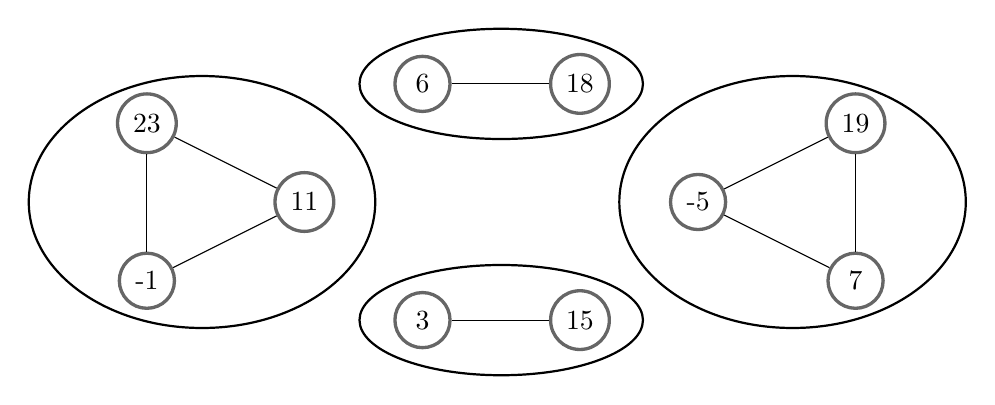
\begin{tikzpicture}[
    node/.style={circle, draw=black!60, very thick, minimum size=7mm},
    ]
    %Nodes
    \node[node] at (-0.5, 0.5) (a) {-1};
    \node[node] at (1.5, 1.5) (b) {11};
    \node[node] at (-0.5, 2.5) (c) {23};
    \node[node] at (6.5, 1.5) (d) {-5};
    \node[node] at (8.5, 0.5) (e) {7};
    \node[node] at (8.5, 2.5) (f) {19};
    \node[node] at (3, 0) (g) {3};
    \node[node] at (5, 0) (h) {15};
    \node[node] at (3, 3) (i) {6};
    \node[node] at (5, 3) (j) {18};
    
    %Lines
    \draw[-] (a) -- (b);
    \draw[-] (a) -- (c);
    \draw[-] (b) -- (c);
    \draw[-] (d) -- (e);
    \draw[-] (d) -- (f);
    \draw[-] (e) -- (f);
    \draw[-] (g) -- (h);
    \draw[-] (i) -- (j);
    
    %elipses
    \draw[thick] (4,0) ellipse (1.8 and 0.7);
    \draw[thick] (4,3) ellipse (1.8 and 0.7);
    \draw[thick] (0.2,1.5) ellipse (2.2 and 1.6);
    \draw[thick] (7.7,1.5) ellipse (2.2 and 1.6);
\end{tikzpicture}
\end{center}
\end{vis}

\subsection{Type-Theoretic view}
This paper focuses on the implementation of quotient types in Coq. Thus, we focus on the Type Theory view of this concept. In Type Theory, quotient types are also induced by some equivalence relation ($\sim$) on underlying type $T$ and denoted $T/\sim$. We denote the equality of elements in the quotient type $T/\sim$ as $a =_\sim b$. Two elements $a$ and $b$ are equal ($a =_\sim b$) if and only if they are in relation ($a \sim b$). Every element of underlying type $T$ is also an element of quotient type $T/\sim$.

Nevertheless, only some functions from underlying type $T$ are well-defined from type $T/\sim$. Function $f : T \rightarrow X$ is well-defined function $f : (T/\sim) \rightarrow X$, if $a \sim b$ implies that $f(a) = f(b)$. Without this restriction, we could differentiate between elements of this same equivalence class by applying an ill-defined function. In other words, applying an ill-defined function breaks the rule that says: $x = y \Rightarrow f(x) = f(y)$.

\section{Quotient types in Coq}
As we mentioned previously, Coq has no built-in method for quotient constructions. Nevertheless, quotients are a helpful concept in formalizing mathematics. Moreover, quotient data types such as sets and multisets are used in many algorithms. Therefore since Coq was introduced, users have been looking for ways to deal with quotients in the Coq language \cite{cicQuotient} \cite{PragmaticQT} \cite{NormalizedTypes}. From those studies, two ways of working with quotient-like types emerged. The first one focuses on replacing the equality relation with an equivalence relation. The second focuses on changing the underlying type so that equivalence implies equality. Both approaches have their downsides and are used interchangeably depending on the situation. In this paper, we focus on the second approach.

\subsection{The setoid approach}
\begin{defi}{Setoid}{def:setoid}
In mathematics, a \emph{setoid} is a set $A$ with an equivalence relation ($\sim$). It is denoted as $(A, \sim)$. In setoids, relation ($\sim$) is meant to be used in place of equality on set A.
\end{defi}
Setoids are concepts known from type theory \cite{SetoidsInTT} \cite{Setoids2}. In Coq, they are often used in the formalization of mathematical concepts. When working with setoids, we need to replace the equality relation in the theorem we are proving with the equivalence relation of the setoid we want to use. It is a minor inconvenience. The bigger one occurs when we want to apply a function on an element of our setoid. In this case, we need to prove that function that is applied is well-defined on setoid (respects equivalence relation). Coq standard library has tools to help users use setoids like rewriting parts of equivalent statements. Unfortunately, it is still far more problematic than using simple equality.

\subsection{The type-based apprach}
Another approach to the lack of quotients in Coq is to define certain types 
where equivalence is the same as equality. This approach usually involves reducing the size of each equivalence class to a single element.

\subsubsection{Subtyping}
This concept will be discussed later in Chapter 2, so the formal definition will be skipped here. Its main idea is to construct a type containing a specific subset of elements. Those elements need to satisfy a particular predicate in case of quotients predicate of being normalized.

\subsubsection{A tailor-made inductive type}
This approach usually gives the best results but only applies to some quotient types. Chapter 4 will show examples of such types based on traces of normalization function. Unfortunately, no general way of getting such type out of the normalization process was not found.

\subsubsection{Additional axioms}
To the Coq system, we can add axioms, and by doing so, we can define quotients similar to other languages like Lean \cite{lean4}. This particular construction will be shown in Chapter 6. Unfortunately, by adding axioms, we lose the computability of our proofs, but usually, we do not need it. However, we must be careful adding axioms since adding contradiction to the Coq system is easy.
\begin{example}{}{ex:ill_defined_mod2}
When dealing with arithmetic modulo 2, we might be tempted to add the following axiom:
\begin{minted}{coq}
Axiom Modulo2 : forall n: nat, n = S (S n).
\end{minted}
It lets us effortlessly rewrite numbers back to their normalized form. Nevertheless, by mistake, we introduced a contradiction. Let us define a function \mintinline{coq}{isZero}, which returns \mintinline{coq}{true} for zero and only zero. Therefore \mintinline{coq}{true = isZero(0) = } \\ \mintinline{coq}{isZero(2) = false}, since \mintinline{coq}{0 = 2}.
\end{example}

\subsubsection{Private inductive types}
Another way of constructing quotients is to use a private inductive type \cite{PrivetInductive}. By using them, we can define the type on which pattern matching outside the module where they are defined is forbidden. If done correctly, it enables us to create constructions like in example \ref{ex:ill_defined_mod2} without introducing contradiction since a user cannot define ill-defined functions.

\section{The equivalence relation induced by a function}
\begin{theo}{The equivalence relation induced by function}{th:equiv_by_fun}
Every function $h: T \rightarrow B$ induces a specific equivalence relation ($\sim_h$) defined below:
$$ \forall x, y \in T, x \sim_h y \iff h(x) = h(y). $$
Moreover, every function $g: B \rightarrow X$ induces a well-defined function $f : T/\sim_h \rightarrow X$ defined as $f = g \circ h$. 
\end{theo}

\begin{proof}{The equivalence relation induced by a function}{proof:equiv_by_fun}
Proof that ($\sim_h$) is an equivalence relation follows directly from the fact that equality on type $B$ is an equivalence relation. \qed \\ 
Given $a, b \in T$ such that $a \sim_h b$. By definition of ($\sim_h$) we know that $h(a) = h(b)$ therefore $f(a) = g(h(a)) = g(h(b)) = f(b)$. So $f$ respects relation $\sim_h$. \qed
\end{proof}
\subsection{Definition of normalization function}
This paper focuses on the particular case of the function $h: T \rightarrow T$, which is idempotent. Such functions we call normalization functions.
\begin{defi}{Normalization function}{def:normalization_function}
\begin{minted}{coq}
Class normalization {A: Type} (f: A -> A) := 
  idempotent : forall x: A, f (f x) = f x.
\end{minted}
\end{defi}
As we know, equivalence relations partition elements into equivalence classes. A normalization function selects a single element from each equivalence class. Elements that have been selected are referred to as normalized or elements in normal form. The idempotence restriction is required to ensure that the normalization function does not change elements already in normal form.

\begin{vis}[B]{Normalization function}{vis:normalization_fuction}
Example of applying normalization function on rational numbers represented as $\mathbb{Z} \times \mathbb{N}$:
\begin{center}
    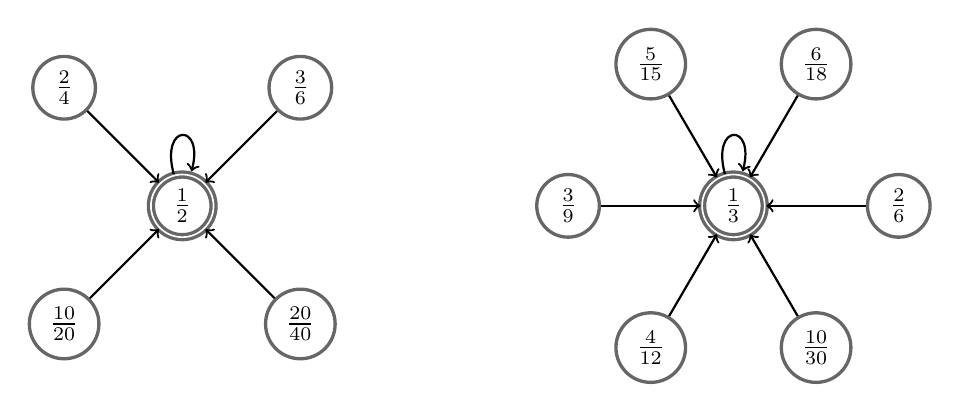
\begin{tikzpicture}[
    node/.style={circle, draw=black!60, very thick, minimum size=0.4}
    ]
    
    %Nodes
    \node[node, double] at (2, 2) (a) {$\frac{1}{2}$};
    \node[node] at (0.5, 3.5) (a0) {$\frac{2}{4}$};
    \node[node] at (3.5, 3.5) (a1) {$\frac{3}{6}$};
    \node[node] at (0.5, 0.5) (a2) {$\frac{10}{20}$};
    \node[node] at (3.5, 0.5) (a3) {$\frac{20}{40}$};

    \node[node, double] at (9, 2) (b) {$\frac{1}{3}$};
    \node[node] at (11.1, 2) (b1) {$\frac{2}{6}$};
    \node[node] at (6.9, 2) (b2) {$\frac{3}{9}$};
    \node[node] at (7.95, 0.2) (b3) {$\frac{4}{12}$};
    \node[node] at (7.95, 3.8) (b4) {$\frac{5}{15}$};
    \node[node] at (10.05, 0.2) (b5) {$\frac{10}{30}$};
    \node[node] at (10.05, 3.8) (b6) {$\frac{6}{18}$};
    
    %Lines
    \path[->, thick] (a) edge [loop above] node {} (a);
    \draw[->, thick] (a0) -- (a);
    \draw[->, thick] (a1) -- (a);
    \draw[->, thick] (a2) -- (a);
    \draw[->, thick] (a3) -- (a);
    
    \path[->, thick] (b) edge [loop above] node {} (b);
    \draw[->, thick] (b1) -- (b);
    \draw[->, thick] (b2) -- (b);
    \draw[->, thick] (b3) -- (b);
    \draw[->, thick] (b4) -- (b);
    \draw[->, thick] (b5) -- (b);
    \draw[->, thick] (b6) -- (b);
    \end{tikzpicture}
\end{center}
\end{vis}

\subsection{Examples of normalization functions}
\begin{example}{Rational numbers}{ex:normalization_fractions}
The standard representation of rational numbers is $\mathbb{Z} \times \mathbb{N}$. For such representation, we can define elements in normal form as irreducible fractions. Therefore normalization function should reduce the fraction by dividing the numerator and the denominator by their greatest common divisor.
\end{example}
\begin{example}{Unordered pair}{ex:normalization_unordered_pirs}
We can define a normalization function for unordered pairs with linear order defined for the underlying type, for example, pairs of natural numbers. Such a function uses the linear order to sort elements of pair. By doing so, the original order of elements in the pair is lost.
\end{example}
\begin{example}{Integers modulo $n$}{ex:normalization_mod}
The normalization function for numbers in arithmetic modulo $n$ is as we expect the operation of calculating modulo.
\end{example}

\section{Quotient types without a normalization function}
Normalization functions are an excellent tool for defining quotient types. By using them, we can select a representative for each equivalence class. Unfortunately, not every quotient type has a computable normalization function. In Set Theory, with the axiom of choice, we can always select a set of representatives of each equivalence relation. Therefore we can always define the normalization function. In Coq, however, we cannot eliminate constructions based on such axiom to define function. 

\subsection{Unordered pairs}
Unordered pair is one of the most basic quotients for which a normalization function does not exist. At least in the most general case, as we learned earlier, if an underlying type has decidable linear order, we can define such a normalization function. Moreover, for some types like, for example, $\mathbb{N} \rightarrow \mathbb{N}$, it is also possible to create such a normalization function based on the computable minimum and maximum, although linear order is not decidable \cite{DefinableQuotients}.

\begin{theo}{}{th:no_normalization_for_unordered_pair}
There is no function $f: (A \times A) \rightarrow A \times A$ for any type A that, for any $\medcircle , \square \in A$ we have $f((\medcircle , \square)) = f((\square, \medcircle))$ and $\medcircle , \square \in f((\medcircle , \square))$ 
\end{theo}

\begin{proof}{}{proof:no_normalization_for_unordered_pair}
Since $f$ is a function for every type $A$, we cannot use values of $\square, \medcircle$ to determine the order of elements. Therefore there are only two functions: $f((\medcircle , \square)) = (\medcircle , \square)$ and $f((\medcircle , \square)) = (\square , \medcircle)$, that satisfy the second property. As can be easily checked, neither satisfies the first property. \qed
\end{proof}

\subsection{Real numbers represented by Cauchy's sequances}
\begin{defi}{Cauchy sequance}{def:cauchy_seq}
Sequence $\{a_n\}_{n\in \mathbb{N}}$ in called \emph{Cauchy sequance} if  elements become arbitrarily close to each other as the sequence progresses \cite{Anal}.
$$
    \textbf{isCauchy}(a) := \forall \epsilon > 0. \exists N \in \mathbb{N}^+. \forall m, n > N. |a_n - a_m| < \epsilon
$$
\end{defi}
Cauchy sequences are often used to construct real numbers out of rational numbers \cite{CauchyReals}. The issue with this construction is that infinitely (even uncountably) many sequences represent a single real number. Using quotients to fix this problem would give us an excellent representation of real numbers for formalizing mathematics. Unfortunately, there is no computable normalization for Cauchy sequences.

\begin{theo}{}{th:no_normalization_for_reals}
There is no computable function $f: (\mathbb{N} \rightarrow \mathbb{Q}) \rightarrow (\mathbb{N} \rightarrow \mathbb{Q})$ that, for any $a, b \in (\mathbb{N} \rightarrow \mathbb{Q})$ we have $\lim_{n \rightarrow \infty}a_n = \lim_{n \rightarrow \infty}b_n \iff f(a) = f(b)$.
\end{theo}

\begin{proof}[G]{}{proof:no_normalization_for_reals}
Let's assume such function $f$ exists.
Let $s_k$ be a sequence consisting of ones to $k$-th place and zeros after. Let $s_\infty$ be a sequence consisting of all ones. \\For all $k$ limit of $s_k$ is zero, and limit of $s_\infty$ is one. Therefore $f(s_k) \not = f(s_\infty)$. If they are different, that means there is a number $t \in \mathbb{N}$ for which $f(s_k)_t \not = f(s_\infty)_t$. So we are able to differentiate between those two in finite time.\\
Let $M$ be an initial state on the Turing machine. Let $c_M(t)$ be zero if the Turing machine finished computations before $t$-th second and one otherwise. This function is computable for every $M$, so we can apply a function $f$ on it and check if the Turing machine with initial state $M$ holts. But the halting problem is undecidable \cite{Undecidable}, so such function $f$ cannot exist. \contradiction
\end{proof}

\subsection{The delay monad}
\begin{defi}{Delay monad}{def:delay_monad}
\begin{minted}{coq}
CoInductive delayed (A : Type) := Delayed {
  state : A + delayed A
}.
\end{minted}
\end{defi}
The delay monad \cite{DelayedMonad} represents computations that may or may not terminate. It is a valuable concept in Coq since it provides an entirely safe way of implementing functions that may not terminate. We want our normalization function to return a value immediately if the computation ever terminates and return infinite delay otherwise. Unfortunately, similar to Cauchy sequences, such normalization function does not exist.
\begin{theo}{}{th:no_normalization_for_delay_monad}
There is no computable function $f: \textrm{delayed} \; A \rightarrow (A + \textrm{unit})$ that, for any terminating computation, returns its final value. Otherwise, it returns an element of unit type.
\end{theo}
\begin{proof}{}{proof:no_normalization_for_delay_monad}
Let's assume that such function $f$ exists. We can model the computation of every partial computable function using a delay monad. Using the normalization function $f$, we can determine if a partial function terminates. But this makes the halting problem decidable, but we know it is undecidable \cite{Undecidable}. Therefore such a normalization function cannot exist. \contradiction
\end{proof}
